\documentclass[journal]{IEEEtran}
%\usepackage{cite}
% *** GRAPHICS RELATED PACKAGES ***
%
\ifCLASSINFOpdf
  \usepackage[pdftex]{graphicx}
\fi
%
\usepackage[cmex10]{amsmath}


% *** ALIGNMENT PACKAGES ***
%
\usepackage{array}
\usepackage{fixltx2e}

\usepackage{stfloats}
% LaTeX2e). It also provides a command:
\fnbelowfloat

\usepackage{booktabs}
\usepackage{amssymb}
\usepackage{amsmath}
\usepackage{pgf}
\usepackage{tikz}
\usetikzlibrary{arrows,positioning}
\usepackage{url}
\usepackage{color}
\usepackage{graphicx}
\usepackage{xspace}
\newcommand*{\eg}{e.g.\@\xspace}
\newcommand*{\ie}{i.e.\@\xspace}
\newcommand*{\vs}{vs.\@\xspace}

\newcommand*{\EMD}{\mathrm{EMD}}

% correct bad hyphenation here
\hyphenation{wave-let}

\usepackage{color}
\newcommand{\vl}[1]{\textcolor{orange}{Vincent : #1}}
\newcommand{\gl}[1]{\textcolor{red}{Gr\'egoire : #1}}
\newcommand{\ja}[1]{\textcolor{magenta}{Joakim : #1}}
\newcommand{\ml}[1]{\textcolor{blue}{ Mathieu : #1}}

\usepackage[backend=bibtex,style=numeric-comp,sorting=none,firstinits=true]{biblatex}
\bibliography{biblio}
%\renewcommand{\baselinestretch}{2}


\begin{document}
%
% paper title
% can use linebreaks \\ within to get better formatting as desired
% Do not put math or special symbols in the title.
%\title{An evaluation framework for event detection using a morphological model of acoustic scenes}
\title{Auditory Scene Similarity Retrieval and Classification with Relevance-based Quantization of Scattering Features}

\author{Vincent Lostanlen\thanks{This work is supported by the ERC InvariantClass grant 320959.}, Gr\'egoire Lafay, Joakim And\'en, and Mathieu Lagrange}


% make the title area
\maketitle

% As a general rule, do not put math, special symbols or citations
% in the abstract or keywords.
\begin{abstract}

This paper introduces a generic hierarchical modeling scheme for acoustic scenes using the wavelet scattering transform at sub-second time-scales with relevance-based quantization at larger time-scales. Instead of representing a scene using summary statistics, a method popularized by bag-of-features models, each scene is represented by a subset of its most representative features, allowing the retrieval system to focus on discriminative features. We demonstrate the potential of the proposed approach for both acoustic scene similarity retrieval and acoustic scene classification tasks on publicly available datasets, consistently outperforming baseline mel-frequency cepstral coefficient (MFCC) methods.

\end{abstract}

% Note that keywords are not normally used for peerreview paper.
\begin{IEEEkeywords}
acoustic scene classification, acoustic scene segmentation, acoustic scene similarity retrieval, scattering, wavelets, invariance
\end{IEEEkeywords}

% For peer review papers, you can put extra information on the cover
% page as needed:
% \ifCLASSOPTIONpeerreview
% \begin{center} \bfseries EDICS Category: 3-BBND \end{center}
% \fi
%
% For peerreview papers, this IEEEtran command inserts a page break and
% creates the second title. It will be ignored for other modes.
\IEEEpeerreviewmaketitle

\section{Introduction}

\IEEEPARstart{T}{he} amount of audio data recorded from our sonic environment has grown considerably over the past decades.
In order to measure the effect of human activity and climate change on animal biodiversity, researchers in the field of ecoacoustics \cite{krause} have recently undertaken the massive deployment of acoustic sensors throughout the world \cite{warren2006urban, NessSST13, stowell13b}. 
In addition, recent work has explored acoustic monitoring for characterization of human pleasantness in urban areas \cite{guyot2005urban, ricciardi2015sound}, as well as the prediction of annoyance due to traffic \cite{gloaguen}.
Because they bear a strong societal impact and raise many scientific challenges, we believe that these applications are of considerable interest for the signal processing community.

Ecoacoustics is the interdisciplinary study of relationships between natural or anthropogenic sounds and their environments at the intersection of ecology, acoustics and computer science. Despite identified needs, the field of signal-based ecoacoustics is still in its infancy.
As a consequence, few well-designed datasets are readily available for evaluation purposes.

A closely related, and more mature, field of investigation is the classification of acoustic scenes, where the aim is to predict labels by processing audio data.
While narrower in its range of applications, it has the advantage of being rooted in the cognitive psychology of categorization \cite{dubois2006cognitive, guastavino_ideal_2006} and has received the attention of the data mining community for some time, resulting in the availability of well-designed datasets.

Despite the differences, ecoacoustics and acoustic scene classification (ASC) task both raise the following question: how can we efficiently and effectively process a large amount of audio data using representations that are compact, generic in their design, and flexible in their use?
The work described in this paper attempts to answer this question by demonstrating the usefulness of two concepts for environmental audio processing: 1) application of the wavelet scattering transform to extract discriminative features and 2) large time-scale modeling of the acoustic scene based on unsupervised clustering of each acoustic scene, allowing us to focus the scene description on a few salient sound objects that carry most of the semantic information. %\ja{Technically, the 1st concept has already been demonstrated in previous papers. Do we really want to claim this here?} ML narrowed the scope

Motivations of the proposed approach and a brief review of the state of the art in the field of acoustic scene modeling is given in Section \ref{sec:soa}. We describe the scattering transform in Section \ref{sec:scattering}, discuss processing of the resulting features in Section \ref{sec:design} and propose a cluster-based scene description in Section \ref{sec:object}. In Section \ref{sec:experiments}, several experiments are proposed for the unsupervised setting of acoustic scene similarity retrieval (ASSR) and for the supervised setting of acoustic scene classification (ASC). Results are subsequently reported in Section \ref{sec:results}.

\section{Background} \label{sec:soa}

%One avenue of ecoacoustics research, originating in bioacoustics, attempts to identify species properties of vocalizations, for example to link animal vocalization with behavior\cite{au2008principles, stowell2014large}.

Computational bioacoustics usually refers to the investigation of sound production, dispersion and reception in animals (including humans) by computational means. A recent paradigm  processes the audio stream in a holistic way over large time-scales, without assuming that a single species is present throughout the recording. Automated systems belonging to this paradigm attempt to infer global properties of bioacoustic scenes, including biodiversity indices \cite{Bardeli2010}, migration patterns \cite{Obrist2010}, as well as marking time intervals of particular interest for detailed human inspection \cite{rosenstock2002landbird}.

%The same division is found in the field of auditory scene analysis, wherein the interest may either be 1) to isolate and identify precise events, \ie acoustic event detection (AED), or 2) to predict global attributes assigned to large time spans of audio, \ie acoustic scene classification (ASC).
For these tasks, a popular approach is the bag-of-frames (BOF) approach for acoustic scene modeling introduced by Aucouturier et al. \cite{aucouturier2007bag}, where a scene is modeled by high-level summary statistics computed from local features.
Being a very generic method, this approach has been applied to many audio classification tasks besides ASC.
Yet the proposed implementation using Gaussian mixture models (GMMs) of mel-frequency cepstral coefficients (MFCCs) has been demonstrated to perform comparably to a direct averaging of the features for a variety of tasks \cite{lagrange:hal-01082501}.
Indeed, the typical morphology of acoustic scenes is a ``skeleton of events on a bed of textures'' \cite{nelken2013}, with a few discrete sound events superimposed upon a stationary acoustic background.
Therefore, it is arguably more beneficial to focus on characterizing these distinct events through describing the large-scale temporal evolution of auditory scenes rather than on the joint probability distribution of short-term features.

This statement has some support in auditory psychology as well as sound synthesis based on summary statistics \cite{mcdermott2013summary}. For example, studies in the cognitive psychology of urban sound environments have shown that global sound level (perceived or measured) is not sufficient to fully characterize an acoustic scene \cite{guyot2005urban,kang2006urban}. Rather, it seems that cognitive processes such as sound environment quality perception \cite{dubois2006cognitive} or loudness judgment \cite{kuwano_memory_2003} rely upon higher-level cognitive attributes such as the identities of sound sources which compose the scene. It has been shown that, if available, the complete description of the scene in terms of event occurrences is powerful enough to reliably predict high-level cognitive classes. For example, the presence of birds is very likely to be heard in parks in urban areas and so are strong pleasantness indicators. Consequently, research in sound perception is now strongly focused on the contribution of specific sound sources in the assessment of sound environments \cite{ricciardi2015sound,lavandier2006contribution}. Although the complete set of events occurring within a given auditory stream may not be discernable, even to human expects, research has shown that a small set of events, so-called markers, suffice to reliably predict many high-level attributes.

From a cognitive psychology perspective, the consensus is therefore that only a few distinct events are sufficient to describe an auditory scene, in contrast to BOF approaches which treat each observation equally when computing summary statistics. A method that takes this knowledge into account could therefore have potential for great impact in the modeling of acoustic scenes.

Aside from \cite{aucouturier2007bag} and \cite{lagrange:hal-01082501} that consider the task of ASSR, much of the work dedicated to acoustic scene modeling is applied to the ASC task.
An overview of the efforts for the latter task is provided by the IEEE Audio and Acoustic Signal Processing (AASP) Detection and Classification of Acoustic Scenes and Events (DCASE) challenge \cite{barchiesi2015acoustic}, held in 2013 to compare different approaches to scene classification. Table \ref{tab:dcase} summarizes the results of the submitted algorithms as well as newer systems that use the private part of the DCASE 2013 dataset for their experiments. Most of the scene prediction results are achieved by majority voting of predictions over local features.

\begin{table}
\begin{center}
\caption{Algorithms evaluated on the DCASE 2013 private dataset of acoustic scene classification. Algorithms above the horizontal line participated to the DCASE challenge. The algorithm marked with $^*$ considered only the public dataset. \label{tab:dcase} \ml{need to define RQA ILD LDA or remove table ?} %\ja{What are the initials OE, ELF, etc. for? Do we need them?}
}
\begin{tabular}{lcl}
& Acc. \%  &  \multicolumn{1}{c}{Design}  \\
\hline
\cite{olivetti2013wonder} & 17 & compression distance, random forests \\
\cite{elizalde2013vector} & 55 & i-vector, LDA \\
\cite{krijnders2013tone} & 55 & cochleogram, SVMs \\
\cite{patil2013multiresolution} & 58 & 2D Gabor filters, SVMs \\
\cite{lee2013acoustic} & 60 & unsupervised learning over mel spectra, SVMs \\
\cite{nogueira2013sound} & 60 & MFCCs and ILD features, SVMs \\
\cite{chum2013ieee} & 65 & sparsity features, HMMs  \\
\cite{geiger2013large} & 69 & mel spectra and MFCCs, SVMs \\
\cite{rakotomamonjy2015histogram} & 69 & histogram of gradient (HOG), SVMs \\
\cite{li2013auditory} & 72 & MFCCs, tree baggers \\
\cite{roma2013} & 76 & RQA features stacked with MFCCs, SVMs \\
\hline
\cite{phan2016label} & 84/87 & label tree embedding of Gammatone, SVMs \\
\cite{7362846} & 85$^*$ & amplitude modulated spectra, LDA \\
\end{tabular}
\end{center}
\end{table}

%\gl{Othe this r paper:} \cite{jiang2005svm, kalinli2009saliency, su2011environmental, ye2015acoustic, bisot2015hog, chakrabarty2015exploring, xue2015auditory}

%\subsection{Datasets}

 % The latter is also considered in this paper as a validation of the proposed approach. \ja{What does this last sentence mean?}

%In this paper, we shall demonstrate that the use of features based on the wavelet scattering transform together with object-based representation of the acoustic scene allows us to achieve state-of-the-art \ja{?} performance in both the ASSR and ASC paradigms.

\section{Wavelet scattering \label{sec:scattering}}

Scattering transforms are time-shift invariant representations of audio signals computed by applying auditory and modulation filter banks alternated with complex modulus non-linearities.
This section first explains the importance of local invariance to time-shifting and stability to time-warping in the representation of acoustic scenes, then describes how the scattering transform is designed to satisfy these properties while having a high discriminative power.

\subsection{Invariance and stability in acoustic scenes}
The notion of invariance to time-shifting plays an essential role in acoustic scene similarity retrieval as well as acoustic scene classification.
Indeed, recordings may be shifted locally without affecting their original class memberships.
To discard this superfluous source of variability, signals can be mapped to a time-shifting invariant feature space before training the classifier, eliminating the need for this classifier to explicitly learn this invariance and increasing the robustness of its predictions.

Formally, given a signal $\boldsymbol{x}(t)$, we would like its translation $\boldsymbol{x_c}(t) = \boldsymbol{x}(t-c)$ to be mapped to the same feature vector provided that $|c| \ll T$ for some maximum duration $T$ that specifies the extent of the time-shifting invariance. We can also define more complicated transformations by letting $c$ vary with $t$. In this case, we have $\boldsymbol{x_\tau}(t) = \boldsymbol{x}(t-\tau(t))$ for some function $\tau$, which performs a time-warping of $\boldsymbol{x}(t)$ to obtain $\boldsymbol{x_\tau}(t)$. Time-warpings model various changes, such as small variations in pitch, reverberation, and rhythmic organization of events. These make up an important part of intra-class variability among natural sounds, so a representation that has some insensitivity to such transformations would be very advantageous.

The wavelet scattering transform, described below, has both of these desired properties: invariance to time-shifting and stability to time-warping. The stability condition can be formulated as a Lipschitz continuity property, which guarantees that the feature transforms of $\boldsymbol{x}(t)$ and $\boldsymbol{x_\tau}(t)$ are close together if $|\tau'(t)|$ is bounded by a small constant.

\subsection{Wavelet scalogram}
Our convention for the Fourier transform of a continuous-time signal $\boldsymbol{x}(t)$ is $\boldsymbol{\hat{x}}(\omega) = \int_{-\infty}^{+\infty} x(t) \exp(- \mathrm{i} 2\pi \omega t) \; \mathrm{d}t$.
Let $\boldsymbol{\psi}(t)$ a complex-valued band-pass filter of
center frequency $\xi_1$ and bandwidth $\xi_1/Q_1$, where $Q_1$ is the quality factor of the filter.
A filter bank of wavelets is built by dilating $\boldsymbol{\psi}(t)$
according to a geometric sequence of scales $2^{\gamma_1/Q_1}$, obtaining
\begin{equation}
\boldsymbol{\psi_{\gamma_1}}(t) = 2^{-\gamma_1/Q_1} \boldsymbol{\psi}(2^{-\gamma_1/Q_1} t)\mbox{.}
\end{equation}
The variable $\gamma_1$ is a scale (an inverse log-frequency) taking integer values between $0$ and $(J_1 \times Q_1 - 1)$, where $J_1$ is the number of octaves spanned by the filter bank.
For each $\gamma_1$, the wavelet $\boldsymbol{\psi_{\gamma_1}}(t)$
has a center frequency of $2^{-\gamma_1/Q_1}\xi_1$ and a bandwidth of $2^{-\gamma_1/Q_1}\xi_1/Q_1$ resulting in the same quality factor $Q_1$ as $\boldsymbol{\psi}$.
In the sequel, we set $\xi_1$ to $20~\mathrm{kHz}$, $J_1$ to $10$, and the quality factor $Q_1$, which doubles as the number of wavelets per octave, to $8$. This results in the wavelet filters covering the whole range of human hearing, from $20~\mathrm{Hz}$ to $20~\mathrm{kHz}$. Setting $Q_1 = 8$ results in filters whose bandwidth approximates an equivalent rectangular bandwidth (ERB) scale.

The wavelet transform of an audio signal
$\boldsymbol{x}(t)$ is obtained by convolution with all wavelet filters
Applying pointwise complex modulus the transform yields
the wavelet scalogram
\begin{equation}
\boldsymbol{x_1}(t, \gamma_1)
= \vert \boldsymbol{x} \ast \boldsymbol{\psi_{\gamma_1}} \vert (t)\mbox{.}
\end{equation}
The scalogram bears resemblance to the constant-Q transform (CQT),
which is derived from the short-term Fourier transform (STFT) by averaging the frequency
axis into constant-Q subbands of center frequencies $2^{-\gamma_1/Q_1}\xi_1$.
Indeed, both time-frequency representations are indexed by time $t$ and log-frequency $\gamma_1$.
However, contrary to the CQT, the wavelet scalogram reaches the Heisenberg
theoretical limit of optimal time-frequency localization across the whole
frequency range, whereas the temporal resolution of the traditional CQT is fixed by the support of the STFT analyzing window. %\cite{Brown1992}
Therefore, the wavelet scalogram has a better temporal localization at high
frequencies than the CQT, at the expense of a greater computational cost
since the inverse fast Fourier transform (IFFT) routine must be called for each wavelet $\boldsymbol{\psi_{\gamma_1}}$ in the filter bank. \ja{Is the cost really greater?}
However, this allows us to observe amplitude modulations at fine temporal scales in the scalogram, down to $2Q_1/\xi_1$ for $\gamma_1 = 0$, of the order of $1\,\textrm{ms}$ given the aforementioned values of $Q_1$ and $\xi_1$. \ja{Where does the formula $2Q_1/\xi_1$ come from?}

To obtain the desired invariance and stability properties, the scalogram is averaged in time using a lowpass filter $\phi(t)$ with cut-off frequency $1/T$ (and so a duration of approximately $T$), to get
\begin{equation}
\mathbf{S_1}\boldsymbol{x}(t, \gamma_1) = \boldsymbol{x_1}(\cdot, \gamma_1) \ast \phi(t),
\end{equation}
which is known as the set of first-order scattering coefficients. They capture the average spectral envelope of $\boldsymbol{x}$ over scales of duration $T$, with the spectral resolution varying with constant Q, as described above. In this way, they are very closely related to the mel-frequency spectrogram and related features, such as MFCCs.

\subsection{Extracting modulations with second-order scattering}
In auditory scenes, amplitude modulations may be caused by a broad variety of rapid mechanical interactions, including collision, friction, turbulent flow, and so on.
At longer time-scales, they also account for higher-level attributes of sound, such as prosody in speech or rhythm in music.
Although they are discarded while filtering $\boldsymbol{x_1}(t,\gamma_1)$ into a local time-shifting invariant representation $\mathbf{S_1}\boldsymbol{x}(t,\gamma_1)$, they can be recovered by a second wavelet transform followed by a pointwise modulus operator.

We define second-order wavelets $\boldsymbol{\psi_{\gamma_2}}(t)$ in the same way as the first-order wavelets, but with parameters $\xi_2$, $J_2$, and $Q_2$ and so have center frequencies $2^{-\gamma_2/Q_2}\xi_2$ for $\gamma_2$ taking values between $0$ and $(J_2 \times Q_2 - 1)$. While this abuses notation slightly, the identity of the wavelets should be clear from context.
The amplitude modulation spectrum resulting from a wavelet modulus decomposition using these second-order wavelets is then
\begin{equation}
\boldsymbol{x_2}(t,\gamma_1,\gamma_2) =
\vert \boldsymbol{x_1} \ast \boldsymbol{\psi_{\gamma_2}} \vert(t,\gamma_1).
\end{equation}
In the sequel, we set $\xi_2$ to $2.5\,\mathrm{kHz}$, $Q_2$ to $1$, and $J_2$ to $12$. Lastly, the low-pass filter $\phi(t)$ is applied to $\boldsymbol{x_2}$ to guarantee local invariance to time-shifting, which yields
\begin{equation}
\mathbf{S_2}\boldsymbol{x}(t,\gamma_1,\gamma_2) =
(\boldsymbol{x_2}(\cdot,\gamma_1,\gamma_2) \ast \phi)(t).
\end{equation}

The scattering transform $\mathbf{S}\boldsymbol{x}(t,\gamma)$ consists of the concatenation of first-order coefficients $\mathbf{S_1}\boldsymbol{x}(t,\gamma_1)$ and second-order coefficients $\mathbf{S_1}\boldsymbol{x}(t,\gamma_1,\gamma_2)$ into a feature matrix $\mathbf{S}\boldsymbol{x}(t,\gamma)$, where $\gamma$ is a shorthand for either $\gamma_1$ or $(\gamma_1,\gamma_2)$. While higher-order scattering coefficients can be calculated, for the purposes of our current, work, the first and second order are sufficient.

\subsection{Gammatone wavelets}
\begin{figure}
\begin{center}
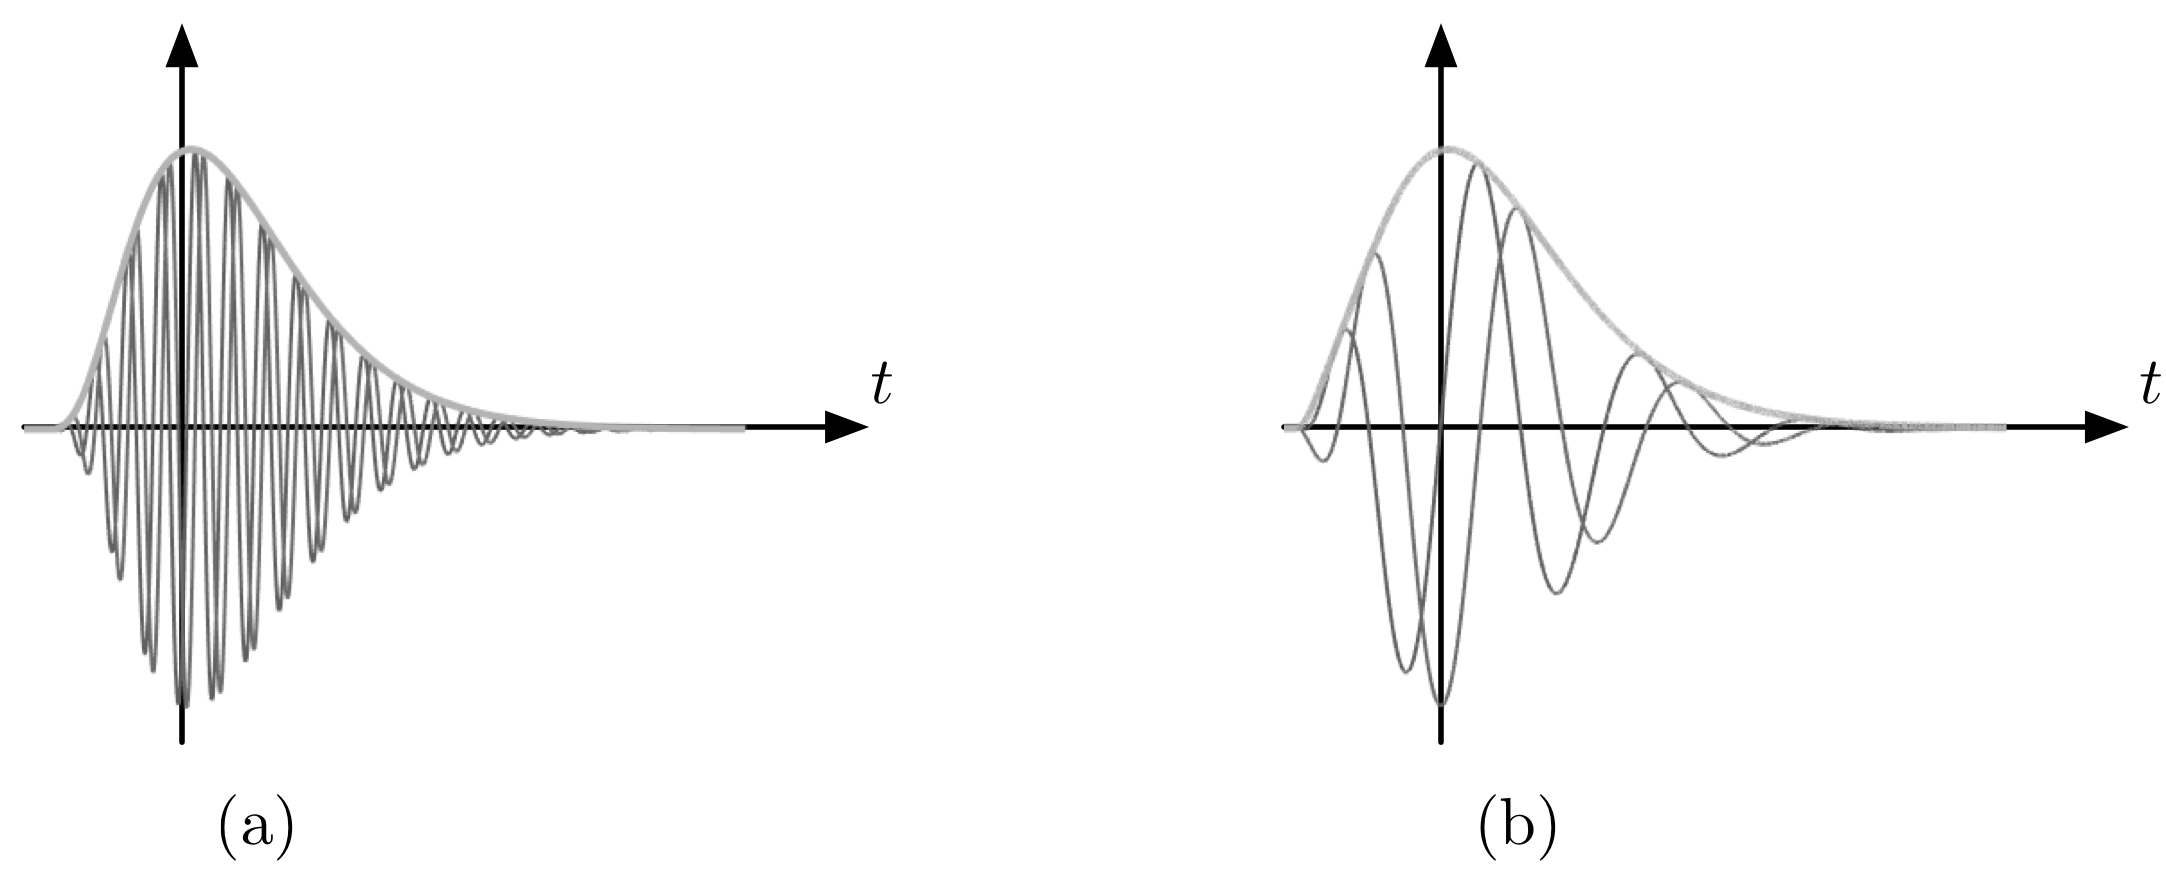
\includegraphics[width=\columnwidth]{bw/gammatones}
\caption{
\label{fig:gammatones}
Gammatone wavelets $\psi(t)$ in the time domain with quality factors (a) $Q = 4$ and (b) $Q = 1$. 
Oscillations represent the real and imaginary parts. The orange envelope represents the complex modulus.}
\end{center}
\end{figure}
Wavelets
$\boldsymbol{\psi_{\gamma_1}}(t)$ and $\boldsymbol{\psi_{\gamma_2}}(t)$ are designed as fourth-order Gammatone
wavelets with one vanishing moment \cite{Venkitaraman2014}, and are shown in Figure \ref{fig:gammatones}.
In the context of auditory scene analysis, the asymmetric envelope of Gammatone wavelets is more biologically plausible than the symmetric, Gaussian-like envelope of the more widely used Morlet wavelets.
Indeed, it allows to reproduce two important psychoacoustic effects in the mammalian cochlea: the asymmetry of temporal masking and the asymmetry of spectral masking  \cite{Fastl2007}.\vl{TODO}
Moreover, it should be noted that Gammatone wavelets follow the typical amplitude profile of natural sounds, beginning with a relatively sharp attack and ending with a slower decay.
As such, they are similar to filters discovered automatically by unsupervised encoding of natural sounds \cite{Smith2006}.
This suggests that, despite being hand-crafted and not learned, Gammatone wavelets provide a sparser time-frequency representation of acoustic scenes compared to other variants.

\section{Feature design}
\label{sec:design}

Before classification or clustering, it is beneficial to process scattering coefficients to improve invariance, normality, and generalization power.
In this section, we review three transformations which achieve these properties, namely logarithmic compression, temporal integration, and standardization.

\subsection{Logarithmic compression}
\label{sec:logcomp}

Many algorithms in pattern recognition, including nearest-neighbor classifiers and support vector machines (SVMs), tend to work best when all features follow a standard normal distribution across all training instances \cite{Hsu2003}.
Yet the distribution of the scattering coefficients is skewed towards larger values. We can reduce this skewness by applying a pointwise concave transformation to all coefficients. In particular, we find that the logarithm performs particularly well in this respect.
Figure \ref{fig:histograms} shows the distribution of an arbitrarily chosen scattering coefficient over the DCASE 2013 dataset, before and after logarithmic compression.

\begin{figure}
\begin{center}
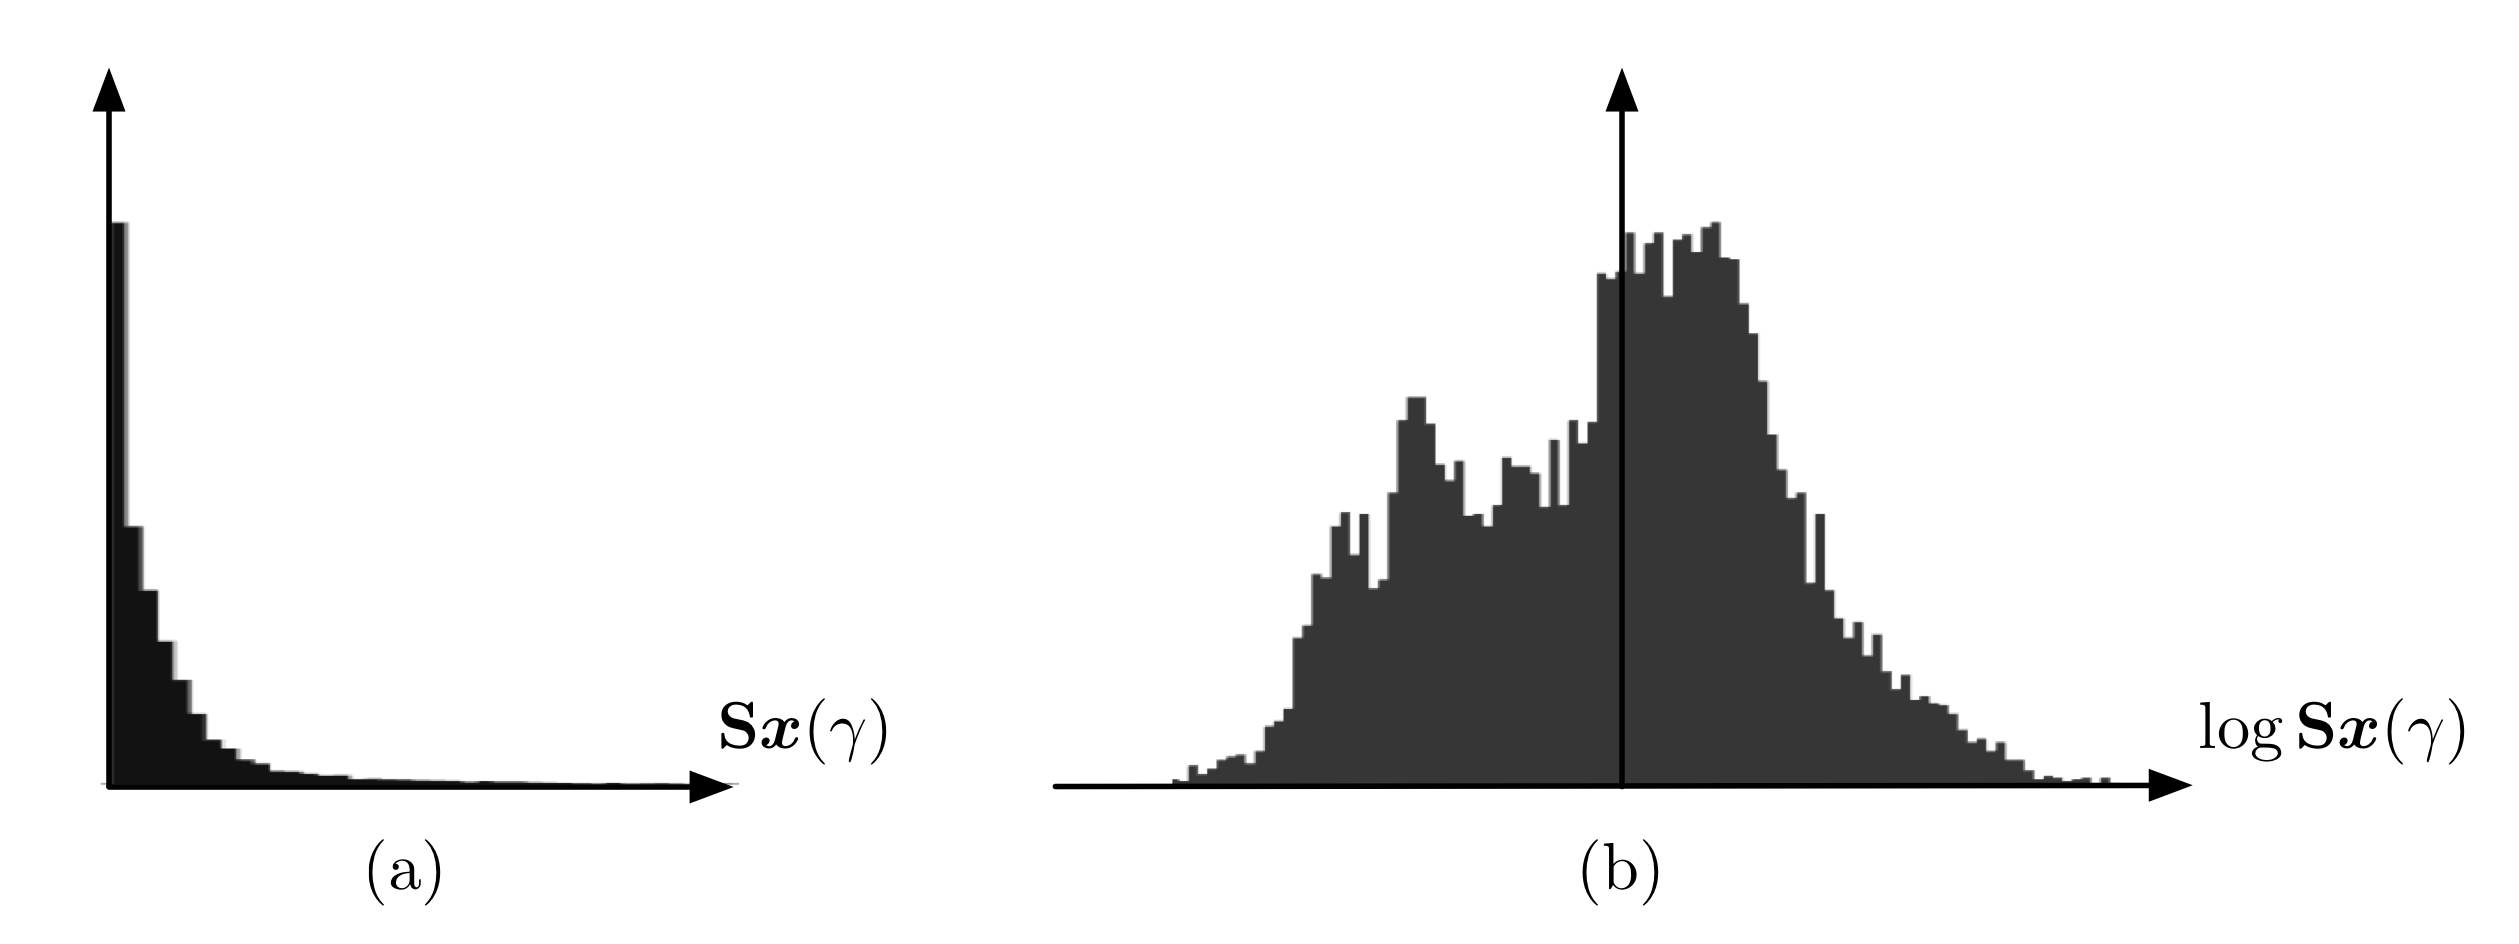
\includegraphics[width=\columnwidth]{bw/compression}
\caption{
\label{fig:histograms}
Histogram of values taken by the first-order scattering coefficient $\mathbf{S}\boldsymbol{x}(\gamma)$, corresponding to a center acoustic frequency of $302\,\mathrm{Hz}$,
(a) before and (b) after logarithmic compression.}
\label{fig:compression}
\end{center}
\end{figure}


Taking the logarithm of a magnitude spectrum is ubiquitous in audio signal processing.
Indeed, it is corroborated by the Weber-Fechner law in psychoacoustics, which states that the sensation of loudness is roughly proportional to the logarithm of the acoustic pressure. 
We must also recall that the measured amplitude of sound sources often decays polynomially with the distance to the microphone--a source of spurious variability in scene classification.
Logarithmic compression linearizes this dependency, facilitating the construction of powerful invariants at the classifier stage.

For the task of musical genre recognition, second-order scattering coefficients $\mathbf{S_2}\boldsymbol{x}(t,\gamma_1,\gamma_2)$ are sometimes normalized by the corresponding first-order scattering coefficients $\mathbf{S_1}\boldsymbol{x}(t,\gamma_1)$, since this decorrelates them from one another \cite{Anden2014}.
We note that taking the logarithm of such renormalized coefficients yields
\begin{equation}
\log \dfrac{\mathbf{S_2}\boldsymbol{x}(t,\gamma_1,\gamma_2)}{\mathbf{S_1}\boldsymbol{x}(t,\gamma_1)} =
\log \mathbf{S_2}\boldsymbol{x}(t, \gamma_1, \gamma_2) -
\log \mathbf{S_1}\boldsymbol{x}(t, \gamma_1),
\end{equation}
\ie a linear combination of the logarithms of first- and second-order coefficients.
As such, a non-linear renormalization becomes a linear transformation, which can be learned by a linearly discriminative classifier. \ja{Do we do this here or not? What is the point of this paragraph?}

\subsection{Early \vs late temporal integration}
\label{sec:eili}

Owing to the scarcity of salient events in many natural scenes,
fine-grained classification is only made
possible by integrating signal information over a long temporal context.
Indeed, whereas a few seconds is often sufficient to recognize a speaker,
a musical instrument, or a genre, up to $30$ seconds may be required
to disambiguate two classes of auditory scenes with overlapping semantic content, \eg a train from a subway station or a quiet street from a park.
Depending on whether aggregation is performed in feature space or in decision space (the output of a classifier) the corresponding method is referred to as early or late integration.

A straightforward application of early integration consists in summarizing the multivariate time series of scattering coefficients over the full duration of the auditory scene by computing their average values over time.
In the definition of the scattering transform (see Section \ref{sec:scattering}), this is equivalent to increasing the support $T$ of the low-pass filter $\boldsymbol{\phi}(t)$ up to infinity. With a slight abuse of notation, we denote the summarized features by
\begin{equation}
\mathbf{S}\boldsymbol{x}(\gamma) =
\int_{-\infty}^{+\infty} \mathbf{S}\boldsymbol{x}(t,\gamma)\;\mathrm{d}t\mbox{.}
\end{equation}

Conversely, a late integration scheme relies on probabilistic assignments $\mathbb{P}\left[y \,\vert\, \mathbf{S}\boldsymbol{x}(t,\gamma) \right]$ over short-term windows of length $T$ obtained from some supervised model, such as a classifier. These are subsequently aggregated to produce a final decision
\begin{equation}
\hat{y} = \arg \max_{y} \rho\Big(\big\{ \mathbb{P}\left[y \,\vert\, \mathbf{S}\boldsymbol{x}(t,\gamma) \right] \big\}_{t} \Big)\mbox{,}
\end{equation}
where $\hat{y}$ is the estimated class label and $\rho$ is a reduction function, such as sum, product, or majority vote \cite{Kittler1998}.

A drawback of early integration is that it drastically reduces the number of training instances at the classifier stage, down to one per auditory scene.
In the context of the DCASE 2013 private dataset, this corresponds to merely $8$ training instances per class, and $80$ instances overall, which can increase the variance of the estimated model and run the risk of overfitting.
On the contrary, once the scattering representation $\mathbf{S}\boldsymbol{x}(t,\gamma)$ has been unpadded of any boundary artifacts, a late integration scheme for $T=372\textrm{ ms}$ would yield $128$ instances per $30$-second auditory scene, resulting in $10240$ instances overall.
However, many of these instances may be silent or lack any salient properties of the class they are assigned to, which may increase the bias in the estimated model and run the risk of underfitting.
Moreover, when applying late integration, the classifier optimizes accuracy at the frame level, not at the scene level, so its prediction might not yield optimal training error under the final evaluation metric.
In short, early and late integration methods lie at opposite ends of the bias-versus-variance statistical tradeoff. The appropriateness of either approach depends therefore on the nature of the signal that is classified.
We refer to \cite{Joder2009} for a comprehensive review of this problematic in the context of musical instrument recognition.
In the context of this paper, early integration refers to an averaging of the features and late integration refers to a majority vote of the predictions given by an SVM. 

\subsection{Standardization}
\label{sec:stand}

Let $\mathbf{S}\boldsymbol{x}(\gamma,n)$ be a dataset, where the $\gamma$ and $n$ respectively denotes feature and sample indices, respectively.
It has been found that SVMs should be trained on scaled features with null mean and unit variance so as to avoid mismatch in numeric ranges \cite{Hsu2003}.
To standardize $\mathbf{S}\boldsymbol{x}(\gamma,n)$, we subtract the sample mean vector $\mu[\mathbf{S}\boldsymbol{x}(\gamma)]$ from $\mathbf{S}\boldsymbol{x}(\gamma,n)$ and divide the result by the sample standard deviation vector $\sigma[\mathbf{S}\boldsymbol{x}] (\gamma)$.
The vectors $\mu[\mathbf{S}\boldsymbol{x}(\gamma)]$ and $\sigma[\mathbf{S}\boldsymbol{x}](\gamma)$ are estimated from the training set only, and the same affine transformation is then applied to all samples in both the training and the test sets.

\section{Relevance based quantization of features}
\label{sec:object}

%As part of the aforementioned research areas and applications, the emerging field of \emph{Acoustic Scene Analysis} (also called \emph{Sound Scene Analysis}) \cite{Stowell15} aims to develop approaches and systems for the automatic analysis of environmental sounds and soundscapes (originating both from urban or nature environments). While research methodologies in related fields such as Automatic Speech Recognition (ASR) \cite{Rabiner93} and Music Information Retrieval (MIR) \cite{Muller07} are now well established, research addressing Acoustic Scene Analysis remains relatively young. 

%From a data processing point of view, a holistic scheme, such as the bag-of-frame approach \cite{aucouturier2007bag}, has a simplicity, but clearly face poor performance on realistic conditions \cite{lagrange:hal-01082501}. 

As discussed in Section \ref{sec:soa}, results in sound perception suggest the appropriateness of source-driven representations of auditory scenes for predicting high-level properties. As the detection of events is still an open problem \cite{7100934}, we consider in this paper a generic quantization scheme in order to identify and represent time intervals of the scene that are coherent, thus likely to be dominated by a given source of interest. \ja{This last sentence is a bit hard to parse. Are we segmenting the time-series and identifying coherent regions?} \ml{better ?}

Given a set of $d$-dimensional feature vectors $X_u = \{x_1^u, \ldots, x_L^u\}$, extracted from the scene $s_u$, where $u=\lbrace 1,2,\ldots,U\rbrace$, we would like to partition $X_u$ into a set $C_u = \{c^u_1, \ldots, c^u_M\}$ of $M$ clusters. The partitioning is done by minimizing squared error between the empirical mean, or centroid, of each cluster and the vectors belonging to it. Letting $\mu_m^u$ denote the centroid of the cluster $c_m^u$, we attempt to minimize the following objective function:
\begin{equation}
J(C_u)=\sum\limits_{m} \sum_{x^u_l\in c^u_m} \Vert x_l^u - \mu_m^u \Vert^2\mbox{.}
\end{equation}
This is known as $k$-means clustering.
Each scene $s_u$ is then described by a set of clusters $C_u$. One should note that this quantization approach differs from unsupervised learning schemes such as the ones studied in \cite{bisot2016acoustic}, where the scene features are projected in a dictionary learned from the entire dataset.

%which clusters not over a single scene, but over the whole dataset, and re-projects each scene in the resulting enhanced feature space. \ja{This sentence is also a big unclear.}

Here, with the aim of better balancing the influence of salient sound events and texture-like sounds on the final decision, the similarity between two scenes is computed based on the similarity of their centroids.

The similarity between the scene centroids $\mu_m^u$ over the entire dataset, is computed using a radial basis function (RBF) kernel $K$ combined with the local scaling method proposed in \cite{selfTuneManor2004}:
\begin{equation}
\label{eq:kc}
K_{mn}^{uv} = \exp\left( - \dfrac{\Vert \mu_m^u - \mu_n^v \Vert^2}{\Vert \mu_m^u - \mu_{m,k}^u \Vert \Vert \mu_n^v - \mu_{n,k}^v \Vert} \right).
\end{equation} 
Here, $\mu_{m,k}^u$ and $\mu_{n,k}^v$ are the $k^{\textrm{th}}$ nearest neighbors to the centroids $\mu_m^u$ and $\mu_n^v$, respectively, and $\Vert \cdot \Vert$ denotes the Euclidean norm.

To compute the similarity between two scenes, we then consider several centroid-based similarity metrics:
\begin{itemize}
\item \emph{ob-closest} (\emph{ob-c}): the similarity between two scenes $s_u$ and $s_v$ is equal to the largest similarity between their centroids, that is
\begin{equation}
	\max_{m,n} K_{mn}^{uv},
\end{equation}
\item \emph{ob-averaged} (\emph{ob-a}): the similarity between two scenes $s_u$ and $s_v$ is equal to the average of their centroid similarities, that is
\begin{equation}
	\frac{1}{M^2} \sum_{m,n} K_{mn}^{uv}
\end{equation}
and,
\item \emph{ob-weighted} (\emph{ob-w}): the similarity between two scenes is computed using a variant of the earth mover's distance applied to the set of centroids weighted by the number of frames assigned to its cluster.
\end{itemize}

For \emph{ob-w}, each centroid is weighted according to the number of frames belonging to its cluster. Each scene $s_u$ is thus described by a signature $p_u$ of $M$ clusters, where $p_u=\lbrace(\mu_1^u,w_1^u),(\mu_2^u,w_2^u),\ldots,(\mu_M^u,w_M^u)\rbrace$) and $\mu_m^u$ and $w_m^u$ are the centroid and the weight of the $m$th cluster, respectively. The similarity between scenes is then given by a cross-bin histogram distance known as the non-normalized earth mover's distance ($\widehat{\EMD}$) introduced by \cite{pele2008linear}. The $\widehat{\EMD}$ computes the distance between two histograms by finding the minimal cost for transforming one histogram into the other, where cost is measured by the number of transported histogram counts times the ``ground distance'' moved in terms of the histogram bins. In our case, the histogram counts are the clusters weights $w_m^u$ defined over the bins formed by the centroids $\mu_m^u$, so the ground distance is the distance over these cluster centroids.

To compute the $\widehat{\EMD}$, we use the implementation proposed in \cite{pele2009fast}. Given two signatures $p_u$ and $p_v$, the $\widehat{\EMD}$ is computed by solving the following linear program:
\begin{equation}
\begin{split}
\widehat{\EMD}(p_u,p_v) &=\left( \min\limits_{\lbrace f_{nm}\rbrace} \sum\limits_{n,m} f_{nm}D_{nm}^{uv} \right) \\
&+ \left|\sum\limits_{n} w_n^u - \sum\limits_{m} w_m^v  \right| \alpha \max\limits_{n,m}\lbrace  D_{nm}^{uv}\rbrace.
\end{split}
\end{equation}

\begin{equation*}
\mathrm{s.t.} \quad f_{nm}\geq0 \quad \sum\limits_{m} f_{nm} \leq w_n^u \quad \sum\limits_{n} f_{nm} \leq w_m^v
\end{equation*}

\begin{equation*}
\sum\limits_{n,m}f_{nm} = \min\left( \sum\limits_{n} w_n^u ,\sum\limits_{m} w_m^v \right)
\end{equation*} 
%\ja{Can we provide some interpretation for the different terms and constraints here?}
where $\lbrace f_{nm} \rbrace$ is the flow between the cluster weights $w_n^u$ and $w_m^v$, that is, the amount transported from the $n^{\textrm{th}}$ bin to ``supply the demand'' of the $m^\textrm{th}$ bin, and $\alpha$ is a parameter which trades off between \ja{?}. We denote by $D^{uv}$ the ground distance, a matrix containing the pairwise distances between the centroids sets $\mu^u$ and $\mu^v$. $D^{uv}$ is computed from the kernel $K$:
\begin{equation*}
D_{mn}^{uv}=1-K_{mn}^{uv}.
\end{equation*}
As suggested in \cite{pele2009fast}, we set the tradeoff parameter $\alpha$ to $1$.

To get the final similarity measure between the scenes $s_u$ and $s_v$, an extended Gaussian kernel $K^s$ is computed: %\cite{chapelle1999support,jing2003support}
\begin{equation}
\label{eq:ks}
K_{uv}^s = \exp\left( - \dfrac{\widehat{\EMD}(p_u,p_v)}{A} \right) \\
\end{equation}
with $A$ a scaling parameter, set to the mean value of the $\widehat{\EMD}$ between all the scenes. The resulting kernel $K^s$ is known as an $\EMD$ kernel, and it should be noted that there is no guarantee that this kernel is positive definite.

\section{Experiments}
\label{sec:experiments}

\subsection{Datasets}

%For most of the experiments reported in this paper, we will consider the DCASE2013 dataset \cite{giannoulis2013database, 7100934}. Larger datasets exists: the
%Rouen dataset \cite{rakotomamonjy2015histogram} and the public part of the DCASE2016 challenge.%
The experiments in this paper are carried out on the DCASE 2013 \cite{7100934} and DCASE 2016 \cite{Mesaros2016_EUSIPCO} datasets.
The DCASE 2013 dataset consists of two parts, namely a public and a private subset, each made up of $100$ $30$-second recordings of various acoustic scenes. The $100$ recordings are evenly divided into $10$ acoustic scene classes. To build the DCASE 2013 dataset, three different recordists visited a wide variety of locations in Greater London over a period of several months and in each scene recorded a few minutes of audio. No
systematic variations in the recordings covaried with scene
type: all recordings were made under moderate weather conditions, at varying times of day and week, and each recordist recorded each scene type. As a consequence, DCASE 2013 dataset enjoys an interesting intra-class diversity while remaining manageable in terms of size, making it suitable for extensive evaluation of algorithmic design choices \cite{lagrange:hal-01082501}.
In addition, it is still a challenging dataset, with a state-of-the-art system based using handcrafted features as input to SVMs achieving $76\%$ \cite{roma2013} (winner of the DCASE2013 challenge), while recent approaches based on label tree embedding achieve between $84\%$ and $87\%$ on DCASE 2013 depending on the prior knowledge used during training \cite{phan2016label}.

%Recent advances using hierarchical classifier architectures obtain between $84\%$ and $87\%$ on DCASE2013 depending on the prior knowledge used during training \cite{phan2016label}. On the Rouen dataset, the state-of-the-art is currently $95\%$ \cite{bisot2016acoustic}.

The public part of the dataset can used for optimizing the ASC system and the private part used for computing the resulting accuracy using a five-fold cross validation scheme. For this paper, we shall perform our experiments on the private part of the dataset. The folds used are the same as the ones used during the challenge.

The DCASE 2016 dataset has a similar organization, but here we conduct our experiments on the public part of the dataset. \ja{Any more information on this dataset?}

%In this paper, we are interested in evaluating different algorithmic designs leading to different scene models, we therefore resort to straightforward ranking performance measures for the ASSR task. \ja{It's not clear to me how the first part implies the second part here} Similarly, we have picked SVMs as our classifier for the ASC task, since these are a standard tool in the community and allows for us to focus our analysis on the earlier processing stages. Moreover, since MFCCs are well-established features which perform well for these task, we shall include them baseline features in all experiments described in this paper.

\subsection{Feature design}

Experiments are carried out using scattering coefficients as well as baseline mel-frequency cepstral coefficients (MFCCs) as features. For the scattering transform, each $30$-second scene is described by $128$ vectors computed with half-overlapping windows $\boldsymbol{\phi}(t)$ of duration $T=372\,\mathrm{ms}$, for a total of $24\,\mathrm{s}$. In this case, $3$ seconds are discarded at the beginning and end of the scene to avoid boundary artifacts. Experiments are conducted with and without logarithmic compression (see Section \ref{sec:logcomp}).

MFCCs are computed for windows of $50\,\mathrm{ms}$ and hops of $25\,\mathrm{ms}$, with full frequency range. The standard configuration of $39$ coefficients coupled with an average-energy measure performs best in preliminary tests, so we use this in the following. The coefficients are averaged using $250\,\mathrm{ms}$ long non-overlapping windows so that each window represents structures of similar scale to the scattering coefficients.

%. The MFCC vectors within each texture window are then averaged in time. As the \emph{ob} approaches involve a clustering step, we need to ensure that both MFCCs and scattering coefficients have a comparable number of vectors per recording. Thus, $t$ is set to $250\,\mathrm{ms}$, resulting in $120$ MFCCs texture windows per scene.

%\ja{We've tested the impact of the logarithm here, but not of the feature selection or standardization. Should we do this as well? For the feature selection, we did say earlier that we would test its impact.}

\subsection{Methods}

The performance of the temporal scattering transform and the \emph{ob} approaches are assessed in an unsupervised setting (ASSR) and in a supervised setting (ASC). \ja{The \emph{ob} approaches are not really assessed for ASC, though.} \ml{well, we say that this does not work well, no ?}

For ASSR, evaluation is performed on the private part of the DCASE 2013 dataset. The metric used is the precision at rank $k$ ($p@k$), which is computed by taking a query item and counting the number of items of the same class within the $k$ closest neighbors, and then averaging over all query items. \ja{The variable $k$ is used previously, so we should change that.} The $p@k$ is computed for $k=\lbrace 1,\ldots,9\rbrace$, since each class only has $10$ items. Note that a $p@1$ is equivalent to the classification accuracy obtained by the classifier which chooses the label of the closest neighbor for a given item. For each experimental setting, we only report the results obtained with the sets of parameters, \emph{i.e.} the number of clusters $M$ for the \emph{ob} approaches and the scaling parameter $k$ of the RBF kernels (see Eq. \ref{eq:kc}) leading to the best $p@9$. The \emph{ob} approaches are compared to commonly used early integration approach \emph{early}.

%\ja{I'm not sure what this means. Do we fix $m$ and $N$ here for all experiments or do we optimize them over the test data each time? If so, this will bias the results, no?}

\begin{figure}[t]
\begin{center}
\includegraphics[width=.9\columnwidth]{bw/unsupervised_test1}
\caption{Acoustic scene similarity retrieval (ASSR) in the DCASE 2013 private dataset: precisions at rank $k$ ($p@k$) obtained for scattering coefficients, with and without logarithmic compression, as a function of the rank $k$. \ja{Why not \emph{ob-a} here? Also, the relationship between the different approaches for the regular scattering coefficients seems to be inverted with respect to the log-scattering and the previous figure. That is, here we have \emph{early} $>$ \emph{ob-w} $\approx$ \emph{ob-c} instead of \emph{ob-w} $>$ \emph{ob-w} $>$ \emph{early}.}}
\label{fig:ASS_2}
\end{center}
\end{figure}

For ASC, the systems are again evaluated on the private part of DCASE 2013, but here with five-fold stratified cross validation. The folds are identical to those used in the original challenge. In the same way as the majority of the DCASE 2013 participants, we use an SVM for the ASC task, which is a large-margin binary discriminator with tunable regularization of misclassified examples. The slack parameter $C$ is here set to $1$. Optimal parameters (see above) are this time learned on the public part of the DCASE 2013 dataset, also using five-fold stratified cross validation. \ja{Which parameters are these?} For these experiments, both \emph{early} and \emph{late} integration strategies are evaluated (see Section \ref{sec:eili}).

For the \emph{ob} approaches, we use the precomputed kernels described in Section \ref{sec:object}. For both the \emph{early} and \emph{late} methods, a linear kernel as well as an RBF kernel are used. As with the RBF kernels used in the \emph{ob} approaches, the RBF kernel in the SVM is scaled locally using the method proposed in \cite{selfTuneManor2004}. All feature vectors, that is scattering frames, MFCCs and centroids, are standardized prior to be given to the classifier. The standardization is computed with respect to the train/test splits of the cross validation scheme (see Section \ref{sec:stand}).

The clustering for the \emph{ob} methods is done using $k$-means$++$ \cite{arthur2007k}, an augmented version of $k$-means with a more robust initialization procedure. Three numbers of clusters are tested: $8$, $16$ and $32$. The implementation of the presented methods as well as the one of the experimental protocol is available.\footnote{\url{https://github.com/mathieulagrange/paperStructureScene16}} \ja{What is ``the one''?}

\section{Results \label{sec:results}}


\subsection{Acoustic Scene Similarity Retrieval}

This section presents evaluation results for the ASSR settings. The $p@k$ for different settings are shown in Figures \ref{fig:ASS_2} and \ref{fig:ASS_1}, illustrating the effect of the different similarity metrics and the influence of the logarithm, respectively.

\subsubsection*{Role of logarithmic compression}

Outcomes for the scattering with and without logarithmic compression are shown in Figure \ref{fig:ASS_2}. It can be seen that the logarithmic compression strongly improves the results, especially for the \emph{ob} approaches, which perform worse than \emph{early} without the logarithmic compression.

\subsubsection*{MFCC \vs scattering transform}

Irrespective of the rank $k$ considered, best result is achieved for the scattering transform with logarithmic compression using the \emph{ob-c} approach. Overall, log-compressed scattering coefficients systematically outperform MFCCs. This is to be expected since the scattering coefficients capture larger-scale modulations, as opposed to MFCCs which only describe the short-time spectral envelope.

\subsubsection*{Relevance-based quantization \vs early integration}

For the scattering transform, both \emph{ob-c} and \emph{ob-w} outperform \emph{early}, thus confirming the benefits of using an relevance-based quantization to improve the similarity measures between the scenes. However, it is worth noticing that \emph{ob-a} performs comparably to \emph{early}, showing that the discriminant information is destroyed by averaging the contributions from all centroids. To take advantage of an such a representation, we need to select certain representative centroids when comparing quantized objects. Furthermore, it appears that \emph{ob-c} is better able to characterize the classes than \emph{ob-w}. This last observation suggests that weighting a centroid according to the number of frames it contains may prove to be a limited solution. Indeed, nothing a priori indicates that the discriminant information between two scenes lays within the majority of their frames. On the contrary, two similar environments may shared a lot of similar sound sources with only a few sources discriminating between them.

The same observations are made for the MFCCs for $k\leq5$. However for a rank $k$ greater than $5$, all the \emph{ob} approaches perform equivalently. This may be due to the fact that, at some point, the MFCCs fail to dissociate the discriminative events of a scene from the non-informative ones, thus making the cluster selection/weighting step useless. \ja{What is the ``at some point'' referring to? In other words, why do we expect this to happen for larger $k$ but not smaller?}
	
%However for a rank $k$ greater than $5$, there is no clear evidence that \emph{ob-c} and \emph{ob-w} approaches improve the results compared to \emph{early}. The latter even outperforms \emph{ob-a} for $k\geq5$. From this it appears that, although the \emph{ob} approaches are able to better retrieve the similarities between close scenes compared to \emph{early}, they are of no help when considering distant scenes of the same class. This may be due to the fact that, at some point, the MFCCs fail to dissociate the discriminative events of a scene from the non-informative ones, thus making a centroid-based description useless, or even counterproductive when the centroids are not weighted/selected.

\begin{figure}[t]
\begin{center}
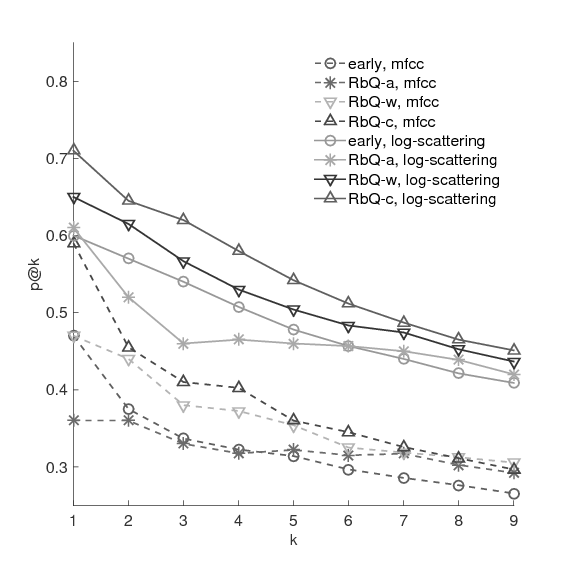
\includegraphics[width=.9\columnwidth]{bw/unsupervised_test2}
\caption{Acoustic scene similarity retrieval (ASSR) in the DCASE 2013 private dataset: precisions at rank $k$ ($p@k$) obtained for MFCCs and scattering with logarithmic compression, as a function of the rank $k$.}
\label{fig:ASS_1}
\end{center}
\end{figure}

\subsection{Acoustic Scene Classification}


\begin{figure}
\begin{center}
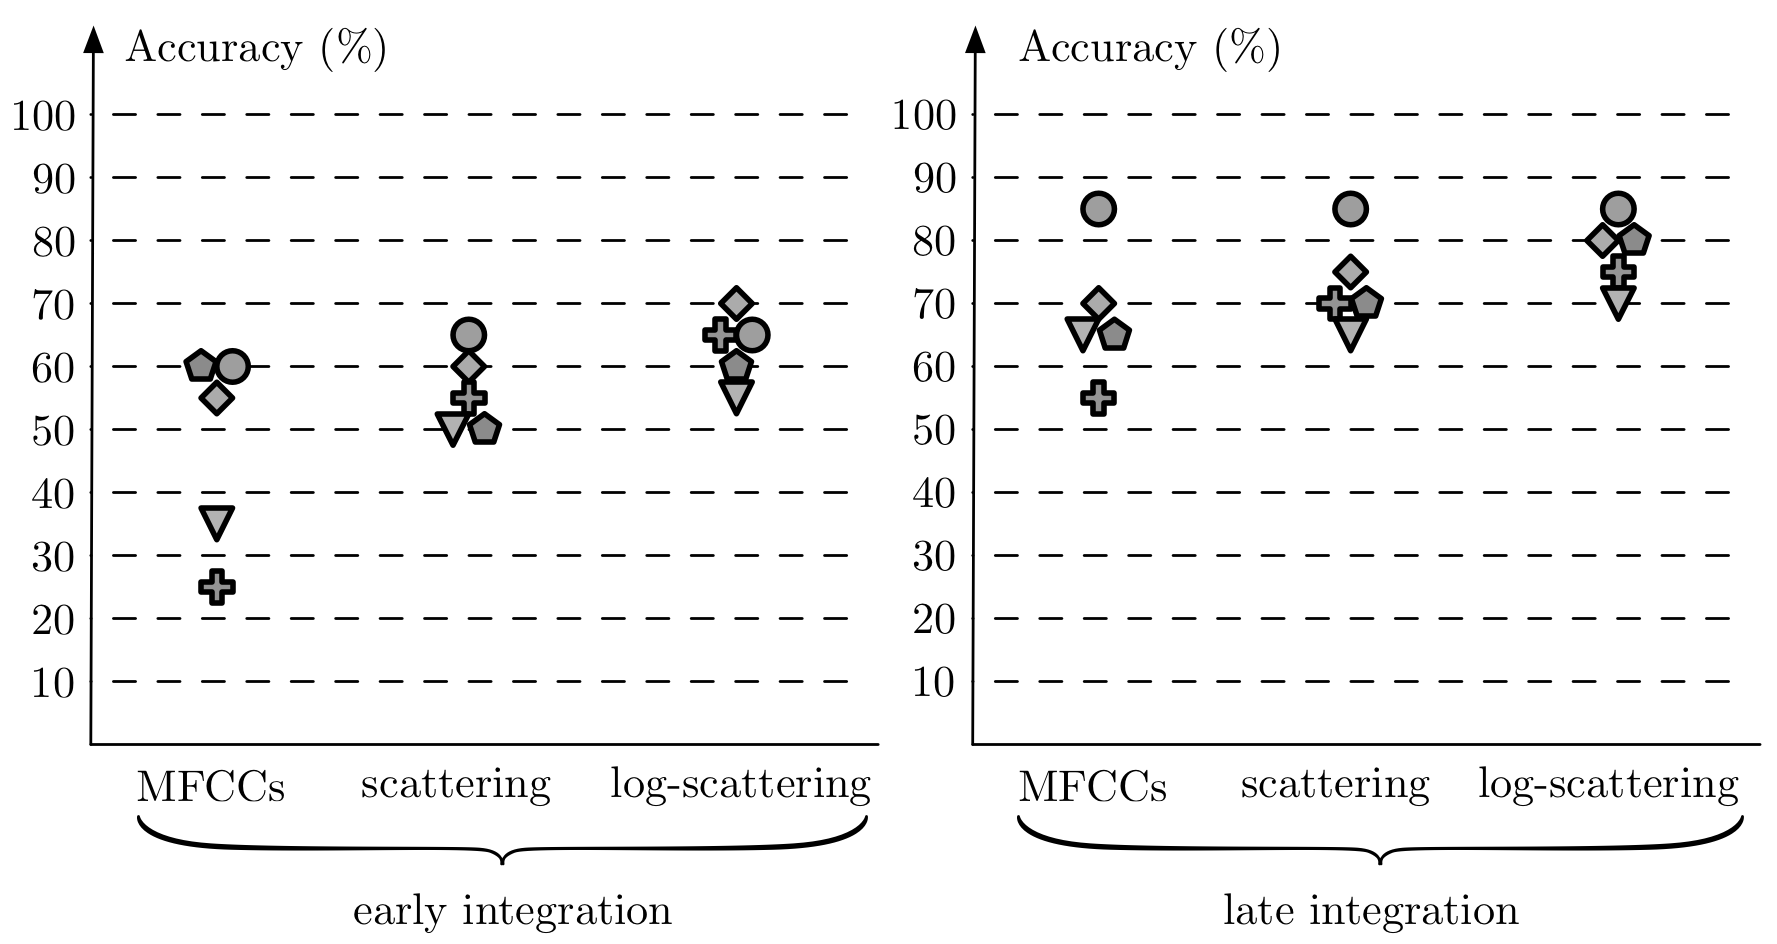
\includegraphics[width=\columnwidth]{bw/folds.png}
\caption{\label{fig:folds}
Classification accuracies over the five folds of the DCASE 2013 private dataset, for various acoustic descriptors and temporal integration strategies.  Performance on each fold is depicted using a given symbol.
The chosen classifier is a support vector machine (SVM) whose kernel is a Gaussian radial basis function (RBF).
The mean accuracies and fold-wise standard deviations of each experiment are reported in Table \ref{table:dcase2013}.}
\end{center}
\end{figure}


We report experiments on acoustic scene classification (ASC), following the original methodology of the DCASE 2013 challenge, and extend our approach to its 2016 edition.

\subsubsection*{MFCCs \vs scattering}

As shown in Figure \ref{fig:folds}, scattering coefficients outperform MFCCs over all but one fold of the DCASE 2013 private dataset when applying early integration, and over all folds when applying late integration.
Not only is the average accuracy improved, but the variance between fold-wise accuracies is also reduced, such as from $16\%$ to $7\%$ in the case of early integration. \ja{Why does this happen?}
This is in accordance with previous results on similarity retrieval, as well as comparisons between mel-frequency coefficients and scattering coefficients for tasks ranging from musical genre recognition and phone segment classification \cite{Anden2014} to environmental sound classification \cite{Salamon2015}.

\subsubsection*{Early \vs late integration}
Late integration, \ie building a prediction by majority voting over $128$ local windows of duration $T=372\,\mathrm{ms}$, outperforms early integration, \ie classifying the acoustic scene with a global window of duration $T=24\,\mathrm{s}$.
This result suggests that, despite its discriminative power at fine scales, the scattering transform is unable to separately characterize distinct acoustic events beyond the scale of about one second. \ja{This is not suggested since the scattering transform is computed at $T=372\,\mathrm{ms}$ and so cannot be expected to capture larger-scale structures. Rather, this says something about the non-stationarity of the audio signals and the fact that we cannot characterize them by some set of summary statistics.}
Therefore, it is beneficial to regard the scattering transform as a mid-level descriptor of acoustic content, not as a high-level descriptor, and adopt a data-driven strategy for the temporal integration of acoustic events within one scene.

Surprisingly, although we ran a large number of experiments to formulate the relevance-based quantization scheme into a supervised setting for acoustic scene classification, none managed to outperform the baseline strategy in \emph{late} temporal integration, namely majority voting. Among such methods, the best result is achieved by the \emph{ob-c} approach with log-compressed scattering coefficients, reaching an accuracy of $66\% \pm0.7$. \ja{Why don't we display these results? Also how is the variance so much smaller here?} \ml{I agree, we should put the results} This might be due to the fact that the discriminability gained by the relevance-based quantization approach is already achieved by the classifiers during training and the fact the relevance-based quantization approach is equivalent to an early fusion approach, which in the case of the DCASE 2013 has not been identified as beneficial due to the dataset size (see discussion in Section \ref{sec:eili}). \ja{This sentence is very confusing.}

\subsubsection*{Role of logarithmic compression}

Logarithmic compression provides a small, albeit consistent boost to acoustic scene classification over all folds in the DCASE 2013 private dataset.
Indeed, as discussed in subsection \ref{sec:logcomp}, and observed in Figure \ref{fig:compression}, the statistical assumption of normality for scattering coefficients is only approximately satisfied once mapped to a logarithmic, decibel-like scale. \ja{Isn't this why we also standardize the coefficients?} \vl{No, standardization does not affect skewness, unlike log compression}
This transformation improves the discriminative power of the SVMs trained on scattering coefficients, regardless of the chosen temporal integration strategy (early or late) and the inner product kernel (linear or Gaussian RBF).
Again, this is in accordance with our previous findings on acoustic scene similarity retrieval, which are reported in Figure \ref{fig:ASS_2}.


\begin{table}
\begin{center}
\caption{
\label{table:dcase2013}
Classification accuracies on the DCASE 2013 dataset with various settings of features, temporal integration strategies, and support vector machine kernels.
\ja{The relationship between linear and RBF is inverted for the \emph{early} integration scheme compared to \emph{late}. Is this correct?}
}
\begin{tabular}{llll}
             & MFCCs         & scattering & log-scattering  \\
             \hline
\emph{early}, linear  & $54\pm20$   & $62\pm\phantom{0}6$  & $66\pm11$     \\
\emph{early}, RBF     & $47\pm16$  & $56\pm\phantom{0}7$  & $63\pm\phantom{0}6$   \\
\emph{late}, linear  & $60\pm\phantom{0}9$ & $70\pm\phantom{0}8$  & $75\pm\phantom{0}5$   \\
\emph{late}, RBF     & $68\pm10$ & $73\pm\phantom{0}8$  & $\mathbf{78}\pm\phantom{0}6$   \\
\end{tabular}
\end{center}
\end{table}

\begin{table}
\begin{center}
\caption{Class-wise accuracies on the DCASE 2016 dataset for the baseline algorithm (left) and proposed algorithm (right).}
\begin{tabular}{lccc}
Features & MFCCs & MFCCs & log-scattering \\
Classifier  & GMMs & linear SVMs & linear SVMs \\
Variant of \emph{late} integration & product & majority vote & majority vote \\
\midrule
beach & $74.6 \pm 18.9$ & $58.3 \pm 28.2$ & $83.5 \pm \phantom{0}7.1$ \\
bus & $58.2 \pm 18.3$ & $58.2 \pm 25.4$ & $88.8 \pm 11.4$ \\
cafe/restaurant & $85.1 \pm 10.8$ & $77.4 \pm 14.7$ & $64.5 \pm \phantom{0}8.3$ \\
car & $69.1 \pm 20.8$ & $92.3 \pm \phantom{0}7.7$ & $94.9 \pm \phantom{0}6.1$ \\
city\_center & $89.6 \pm \phantom{0}9.2$ & $96.4 \pm \phantom{0}3.8$ & $91.7 \pm \phantom{0}9.4$ \\
forest\_path & $72.4 \pm 23.8$ & $67.7 \pm 30.8$ & $93.8 \pm \phantom{0}7.8$ \\
grocery\_store & $74.1 \pm 13.7$ & $44.7 \pm 24.8$ & $90.9 \pm \phantom{0}6.9$ \\
home & $78.1 \pm 17.7$ & $44.8 \pm 15.3$ & $56.2 \pm 23.9$ \\
library & $65.1 \pm 23.3$ & $54.6 \pm 20.3$ & $82.0 \pm 13.0$ \\
metro\_station & $85.2 \pm 15.6$ & $94.7 \pm \phantom{0}6.8$ & $96.0 \pm \phantom{0}2.3$ \\
office & $90.8 \pm 16.0$ & $95.7 \pm \phantom{0}7.5$ & $87.5 \pm 21.7$ \\
park & $25.6 \pm 11.0$ & $52.4 \pm 10.4$ & $75.4 \pm \phantom{0}7.4$ \\
residential\_area & $75.1 \pm 19.4$ & $53.2 \pm 17.0$ & $44.2 \pm 15.0$ \\
train & $34.1 \pm \phantom{0}7.2$ & $44.5 \pm 23.1$ & $58.3 \pm 10.0$ \\
tram & $85.4 \pm 13.9$ & $52.1 \pm 11.9$ & $83.7 \pm 12.2$ \\
\bottomrule
Average & $70.8 \pm \phantom{0}2.6$ & $65.8 \pm \phantom{0}8.0$ & $79.4 \pm \phantom{0}3.0$ \\
\end{tabular}
\end{center}
\label{table:dcase2016}
\end{table}


\subsubsection*{Participation to the DCASE 2016 challenge}
In order to evaluate the generality of our findings, we have taken part in the acoustic scene classification task of the 2016 edition of the DCASE challenge.
This edition relies on the TUT 2016 acoustic scenes dataset, which contains $15$ classes of acoustic scenes, and is larger than the DCASE 2013 private dataset by one order of magnitude \cite{Mesaros2016_EUSIPCO}.
Training support vector machines with a Gaussian RBF kernel is computationally demanding for a dataset of such size, especially under a late integration scheme, wherein the number of training instances exceeds $10^5$, we therefore use a linear kernel instead.
Our experiments on the smaller DCASE 2013 dataset, as reported in table \ref{table:dcase2013}, show that the linear kernel gives comparable, albeit slightly worse, classification results than the Gaussian RBF kernel.

Our results on the public part of the DCASE 2016 dataset are reported in Table \ref{table:dcase2016}, compared with a baseline using MFCCs and a generative classifier, namely Gaussian mixture models with $16$ Gaussians per model. This baseline relies on a late integration scheme, wherein the reduction function $\rho$ is a product of likelihoods. For comparison, we also provide the results for the same MFCC features coupled with a linear SVM classifier. Results here are slightly worse since the SVM can only discriminate between classes that are linearly separable, a limitation not present for the GMMs.

With the scattering transforms, however, the average accuracy across classes is brought from $70.8\%$ to $79.4\%$.\footnote{Challenge results on the private part of the dataset are expected to be published in August 2016.} It is interesting to note, however, that two classes, ``home'' and ``residential\_area'' both drop significantly in accuracy from the baseline GMM model to the scattering SVM classifier. This can be partially explained by the substitution of the GMM with an SVM, which shows a similar drop for the MFCCs. However, another reason could be that these classes are well-characterized by the average spectral envelope of the signal and the second-order modulation information captured by the scattering coefficients is therefore superfluous.
Furthermore, our cross-validation analysis confirmed that the value $T=372\,\mathrm{ms}$ for the support of the low-pass filter $\boldsymbol{\phi}(t)$ is optimal when applying late integration by majority voting.

\section{Conclusion}

In this paper we consider the benefit of 1) the scattering transform for building discriminant features and 2) unsupervised clustering for the modeling of large-scale environmental acoustic scenes.
%This leads to improvements in both the ASSR and ASC tasks.

Representing a scene using a reduced set of representatives, with adapted similarity strategies, allows us to improve ASSR performance compared to the early-integration scheme which have been demonstrated to be equivalent to BOF approaches using GMMs on well-balanced datasets \cite{lagrange:hal-01082501}. These results advocate for a hierarchical model of the scene, where short-time structure--\ie below a second--is represented using a convolutional network such as the scattering transform, whereas larger time scales--\ie over a second--are modeled as adaptive aggregates.

Within a supervised setting of acoustic scene classification (ASC), we have shown the comparative benefits of log-scattering features over MFCCs, of majority voting at a mid-level time scale of $T=372\,\mathrm{ms}$ over prediction at a high-level time scale of $T=24\,\mathrm{s}$, and of an adapted Gaussian kernel over the linear kernel in support vector machine classification for the tasks we considered.
%, identified in the time domain in the unsupervised setting and in the features domain in the supervised case, provided that the dimensionality is sufficiently high. \ja{I'm not sure what this last part means.}

These outcomes shall be studied further in future work by considering larger databases and more diverse applications, such as pleasantness prediction \cite{lafaySoundscapePilot} as well as other emerging tasks in ecoacoustics.

%\bibliographystyle{unsrt}
%\bibliography{biblio}
\printbibliography

\begin{IEEEbiography}[{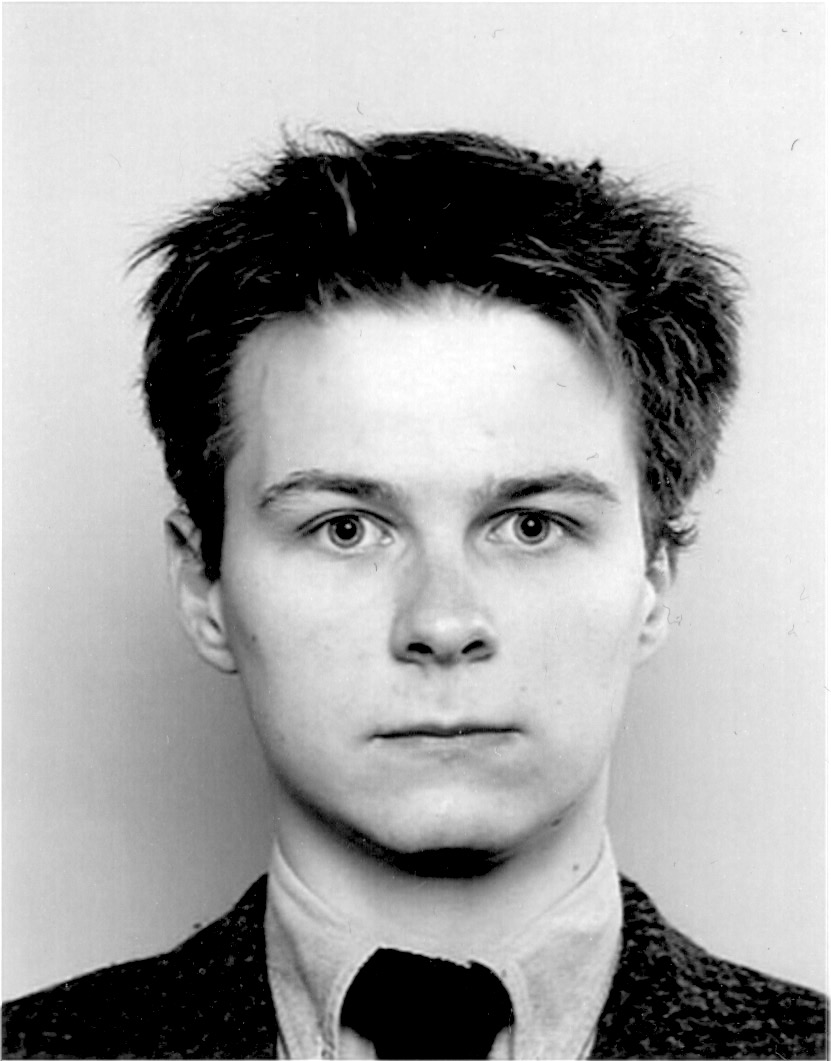
\includegraphics[width=1in,height=1.25in,clip,keepaspectratio]{gfx/lostanlen}}]{Vincent Lostanlen} was born in 1992. He received his M.S. degree in acoustics, signal processing, and musical informatics (ATIAM) from the Universit\'{e} Pierre et Marie Curie and the Ircam in Paris, France, in 2013. Since 2013, he is a PhD student at ENS in Paris.
\end{IEEEbiography}

\begin{IEEEbiography}[{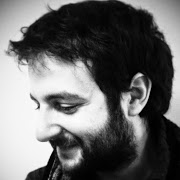
\includegraphics[width=1in,height=1.25in,clip,keepaspectratio]{gfx/lafay}}]{Gr\'egoire Lafay} was born in Paris, France, in 1990. He received in 2011 the B.S. degree in Acoustic from the University Pierre and Marie Curie (UPMC), Paris, France, and the B.S. degree in Musicology from the Sorbonne University, Paris, France. He received his M.S. degree in acoustics, signal processing, and musical informatics (ATIAM) from the Universit\'{e} Pierre and Marie Curie and the Ircam in Paris, France, in 2013. Since 2013, he is a Ph.D student at IRCCyN, a French laboratory dedicated to cybernetics. His current research interests include acoustic scene similarity and classification, as well as acoustic scene perception. 
\end{IEEEbiography}

\begin{IEEEbiography}[{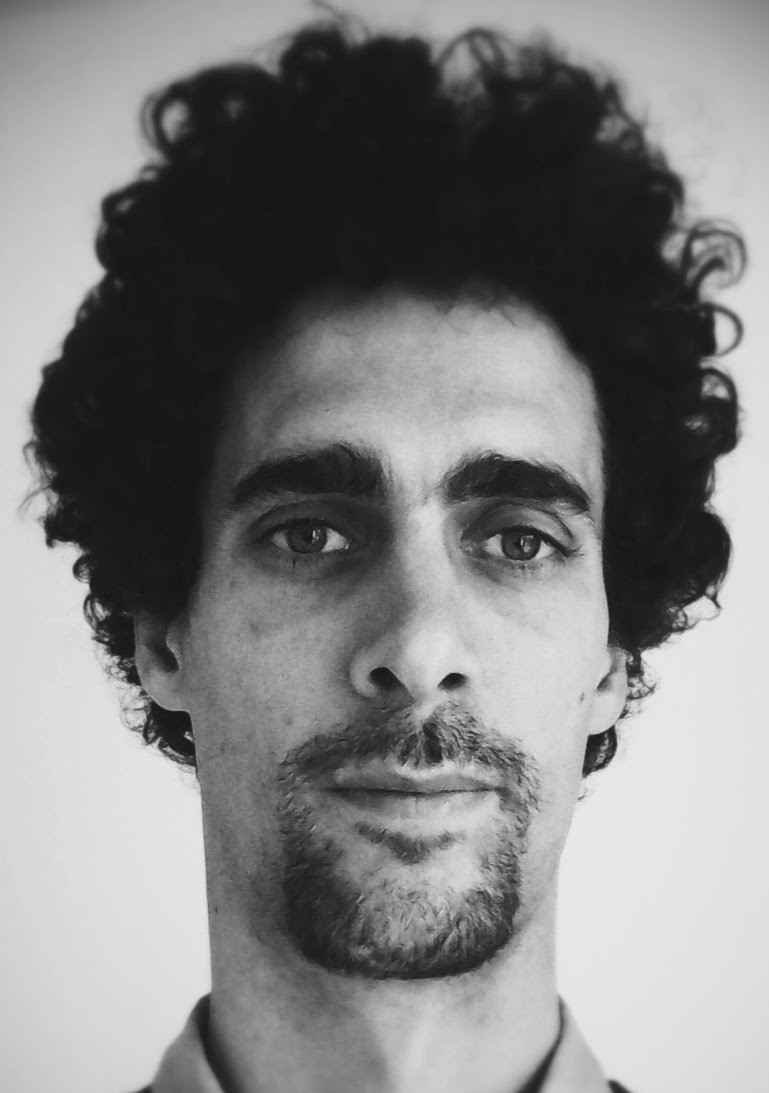
\includegraphics[width=1.25in,height=1.25in,clip,keepaspectratio]{gfx/lagrange}}]{Mathieu Lagrange} is a CNRS research scientist at IRCCyN, a French laboratory dedicated to cybernetics. He obtained his PhD in computer science at the University of Bordeaux in 2004, and visited several institutions in Canada (University of Victoria, McGill University) and in France (Orange Labs, TELECOM ParisTech, Ircam). His research focuses on machine listening algorithms applied to the analysis of musical and environmental audio.
\end{IEEEbiography}

% biography section
% 
% If you have an EPS/PDF photo (graphicx package needed) extra braces are
% needed around the contents of the optional argument to biography to prevent
% the LaTeX parser from getting confused when it sees the complicated
% \includegraphics command within an optional argument. (You could create
% your own custom macro containing the \includegraphics command to make things
% simpler here.)
%\begin{IEEEbiography}[{\includegraphics[width=1in,height=1.25in,clip,keepaspectratio]{mshell}}]{Michael Shell}
% or if you just want to reserve a space for a photo:

%\begin{IEEEbiography}{Mathieu Lagrange}
%Biography text here.
%\end{IEEEbiography}

% if you will not have a photo at all:
%\begin{IEEEbiographynophoto}{John Doe}
%Biography text here.
%\end{IEEEbiographynophoto}

% insert where needed to balance the two columns on the last page with
% biographies
%\newpage

%\begin{IEEEbiographynophoto}{Jane Doe}
%Biography text here.
%\end{IEEEbiographynophoto}

% You can push biographies down or up by placing
% a \vfill before or after them. The appropriate
% use of \vfill depends on what kind of text is
% on the last page and whether or not the columns
% are being equalized.

%\vfill

% Can be used to pull up biographies so that the bottom of the last one
% is flush with the other column.
%\enlargethispage{-5in}



% that's all folks
\end{document}


